\documentclass[a4paper,14pt]{extarticle}
\usepackage[utf8]{inputenc}
\usepackage[russian]{babel}
\usepackage{graphicx}
\usepackage{indentfirst}
\usepackage[top=0.8in, bottom=0.8in, left=0.8in, right=0.8in]{geometry}
\usepackage{pgfplots}
\usepackage{amsmath}
\usepackage{setspace}
\usepackage{titlesec}
\usepackage{subcaption}
\usepackage{float}
\usepackage{chngcntr}
\usepackage{pgfplots}
\usepackage{amsfonts}
\usepackage{hhline}
\usepackage{pgfplotstable}
\usepackage{multirow}
\usepackage{karnaugh-map}
\usepackage{tikz,xcolor}

\titleformat{\section}[hang]
  {\bfseries}
  {}
  {0em}
  {\hspace{-0.4pt}\large \thesection\hspace{0.6em}}
  
  
\titleformat{\subsection}[hang]
  {\bfseries}
  {}
  {0em}
  {\hspace{-0.4pt}\large \thesubsection\hspace{0.6em}}

%\linespread{1.3} % полуторный интервал
%\renewcommand{\rmdefault}{ftm} % Times New Roman

\newcommand{\nx}{\overline{x}}
\newcommand{\p}{0.31}
\newcommand{\scale}{1.4}

\counterwithin{figure}{section}
\counterwithin{equation}{section}
\counterwithin{table}{section}

\begin{document}
\begin{titlepage}
\centering
Санкт-Петербургский политехнический университет Петра Великого \\
Институт компьютерных наук и технологий \\
Кафедра компьютерных систем и программных технологий \\
\vspace{6.0cm}

{\centering \textbf{Отчёт по лабораторной работе №3} \\ 
\vspace{0.15cm}
\textbf{Дисциплина}: Телекоммуникационные технологии \\
\vspace{0.15cm}
\textbf{Тема}: Линейная фильтрация}
\vspace{6.8cm}

\begin{table}[H]
\begin{tabular}{p{\textwidth}@{}r}
{Выполнил студент гр. 33501/4} \hfill { $\underset{\text{(подпись)}}{\underline{\hspace{0.23\textwidth}}}$ Жуйков А.А.} \\
{Преподаватель} \hfill { $\underset{\text{(подпись)}}{\underline{\hspace{0.23\textwidth}}}~~~~$ Богач Н.В.} \\
\vspace{0.15cm}
{} \hfill { <<\underline{\hspace{0.08\textwidth}}>> \underline{\hspace{0.2\textwidth}}2018 г.} \\
\end{tabular}
\end{table}
\vfill
{\centering Санкт-Петербург \\ 
\vspace{0.15cm}
2018}
\end{titlepage}

\section{Цель работы.}
Изучить воздействие ФНЧ на тестовый сигнал с шумом.

\section{Постановка задачи.}
Сгенерировать гармонический сигнал с шумом и синтезировать ФНЧ. Получить сигнал во временной и частотной областях до и после фильтрации. Сделать выводы о воздействии ФНЧ на спектр сигнала.

\section{Теоретические положения.}
\subsection{Линейный дискретный фильтр.}
\textit{Линейный фильтр} -- динамическая система, применяющая линейный оператор ко входному сигналу для выделения или подавления определённых частот сигнала и других функций по обработке входного сигнала. Линейные фильтры широко применяются в электронике, цифровой обработке сигналов и изображений, в оптике, теории управления и других областях.
Наиболее часто они используются для того, чтобы удалить некоторые частоты входного сигнала или для того чтобы выделить необходимую полосу частот в сигнале.

\textit{Линейный дискретный фильтр} – это произвольная система обработки дискретного сигнала, обладающая свойствами линейности и стационарности.

Линейность означает, что выходная реакция на сумму воздействий
равна сумме реакций на эти воздействия, поданные на вход по отдельности.

Стационарность означает, что задержка входного сигнала приводит
лишь к такой же задержке выходного сигнала, не меняя его формы.
В общем случае дискретный фильтр суммирует (с весовыми коэффициентами) некоторое количество входных отсчетов (включая последний) и
некоторое количество предыдущих выходных отсчетов:
\begin{multline*}
y(k) = b_0 x(k) + b_1 x(k-1) + ... + b_m x(k-m) - \\
- a_1 y(k-1) - a_2 y(k-2) - ... - a_n y(k-n), 
\end{multline*}
где $a_j$ и $b_i$ -- вещественные коэффициенты.

Данная формула называется \textit{алгоритмом} или \textit{уравнением дискретной фильтрации}. Записав формулу в другом виде получим \textit{разностное уравнение:}
\begin{multline*}
y(k) + a_1 y(k-1) + a_2 y(k-2) + ... + a_n y(k-n) = \\
= b_0 x(k) + b_1 x(k-1) + ... + b_m x(k-m).
\end{multline*}

\subsection{Нерекурсивный фильтр.}
\textit{Нерекурсивными} называют фильтры, которые не используют предыдущие отсчеты выходного сигнала при вычислении следующих. Уравнение фильтрации принимает вид:
\begin{equation*}
y(k) = \sum_{i=0}^K b_i x(k-i).
\end{equation*}

Количество K используемых отсчетов входного сигнала называется \textit{порядком фильтра}. Импульсная характеристика нерекурсивного фильтра определяется путем подстановки в разностное уравнение единичного импульса $x_0 (k)$ в качестве входного сигнала:
\begin{equation*}
h(k) = \sum_{i=0}^K b_i x_0(k-i) = b_k,
\end{equation*}
т.к. $x_0(k-i) \neq 0$ только для $i = k$.

Таким образом, коэффициенты $b_i$ нерекурсивного фильтра являются
отсчетами его импульсной характеристики. Так как в реальном устройстве
линия задержки содержит конечное число элементов, то импульсная характеристика нерекурсивного фильтра также является конечной по длительности.
Поэтому еще одно название таких фильтров -- фильтры с конечной импульсной характеристикой (КИХ-фильтры, FIR (finite impulse response)).

\subsection{Рекурсивный фильтр.}
Если уравнение фильтрации содержит как входные, так и выходные
отсчеты, то для реализации такого фильтра необходимо добавить вторую
линию задержки - для хранения выходных отсчетов $y(k - i)$.

При вычислениях используются предыдущие отсчеты выходного сигнала, поэтому такие фильтры называют рекурсивными. Уравнение фильтрации может быть записано следующим образом:
\begin{equation*}
y(k) = \sum_{i_0}^K b_i x(k-i) - \sum_{i=1}^N a_i y(k-i).
\end{equation*}
Максимум из чисел $N$ и $K$ называют порядком фильтра.

Так как каждый следующий отсчет импульсной характеристики рекурсивного фильтра вычисляется исходя из значения предыдущего, то количество таких отсчетов не ограничено. Поэтому рекурсивные фильтры называют также фильтрами с бесконечной импульсной характеристикой (БИХ-фильтрами, IIR (infinite impulse response)).

\section{Ход работы.}
\subsection{Генерация сигнала. Наложение шума.}
В среде MATLAB был сгенерирован синусоидальный сигнал $S = \sin(2 \pi f_0 \cdot t)$, представленный на Рис. \ref{clear_sin}.

\begin{figure}[H]
\centering
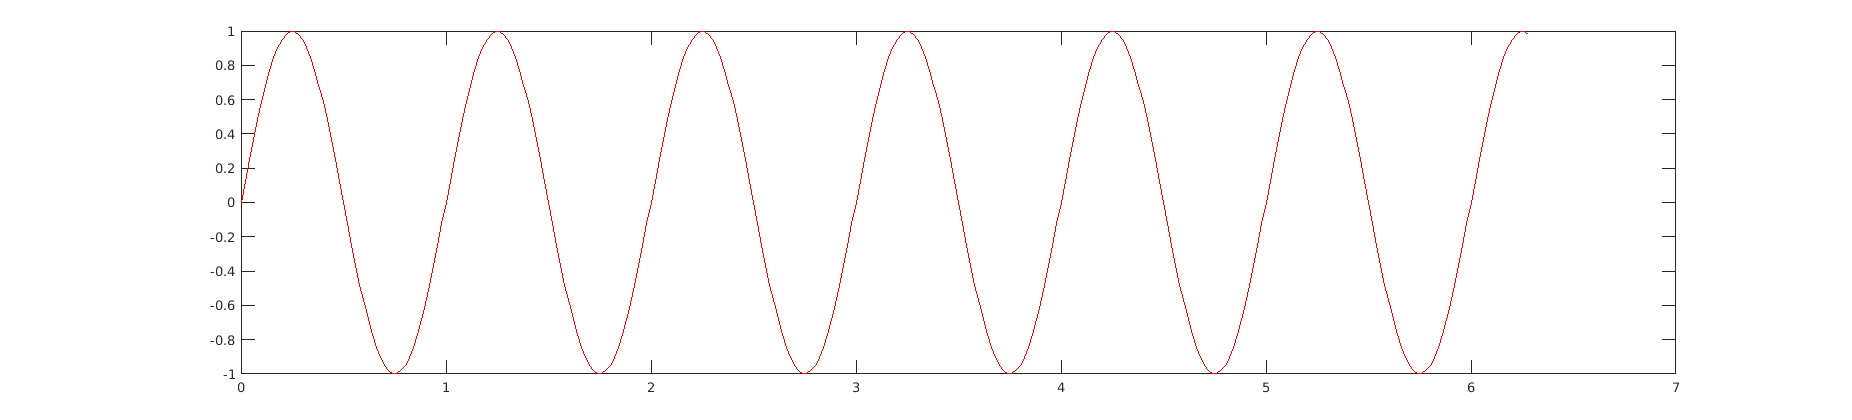
\includegraphics[scale=0.38]{pics/3clear_sin.png}
\caption{Синусоидальный сигнал $S$. $f_0$ = 1 Гц. $f_s$ = 50 Гц.}
\label{clear_sin}
\end{figure}

Для сигнала был получен спектр (Рис \ref{clear_spec}).
\begin{figure}[H]
\centering
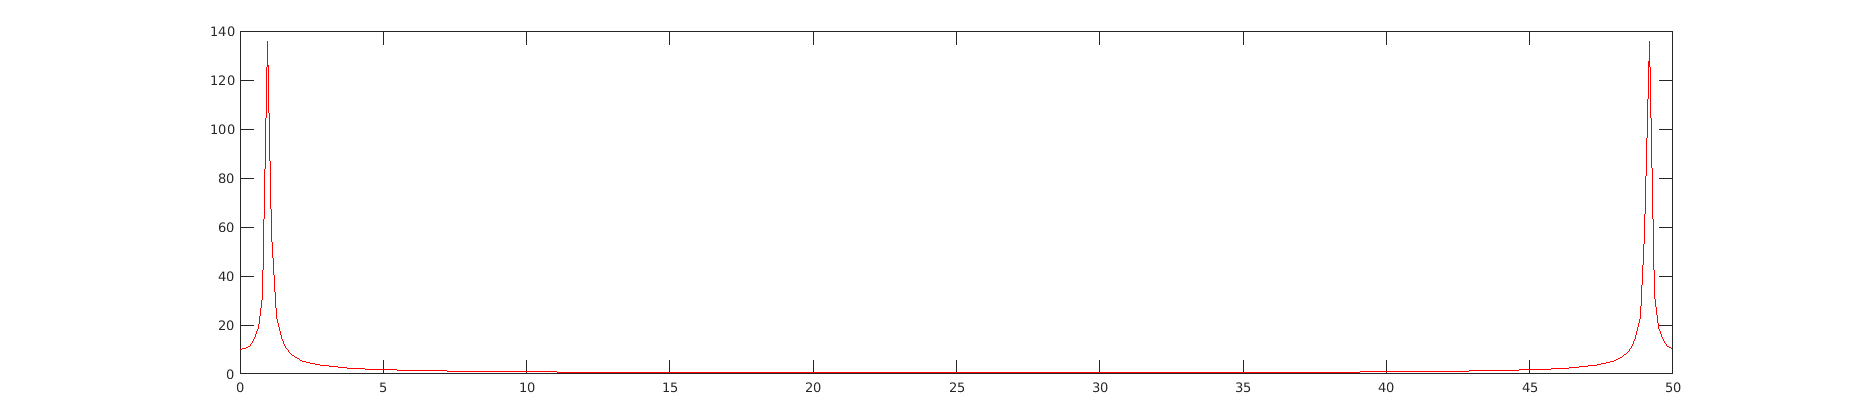
\includegraphics[scale=0.38]{pics/3clear_sin_spec.png}
\caption{Спектр сигнала $S$.}
\label{clear_spec}
\end{figure}

Для добавления шума к сигналу $S$ была использована функция awgn. Функция добавляет к сигналу белый Гауссовский шум. Функция принимает параметр \textit{snr} -- Signal-to-noise Ratio -- отношение сигнала к шуму, выраженное в дБ.  Зашумленный сигнал, а также его спектр представлены на Рис. \ref{noise_sin} и Рис. \ref{noise_sin_spec} соответственно.

\begin{figure}[H]
\centering
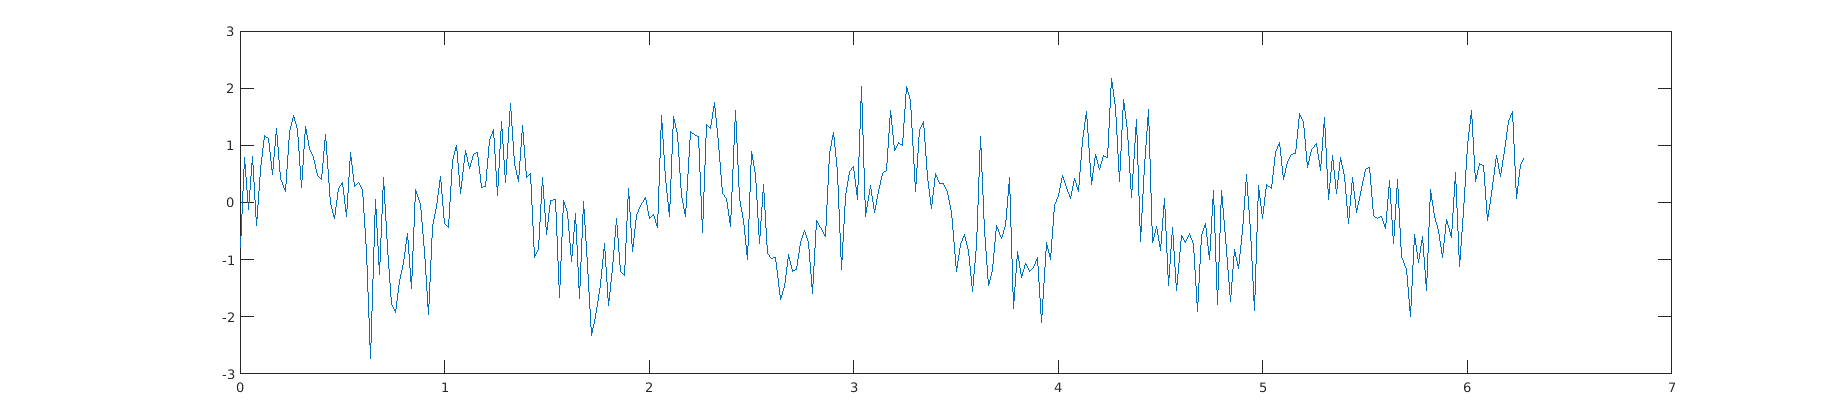
\includegraphics[scale=0.38]{pics/3noise_sin.png}
\caption{Зашумленный сигнал $S$. \textit{signal-to-noise ratio} = 3.}
\label{noise_sin}
\end{figure}

\begin{figure}[H]
\centering
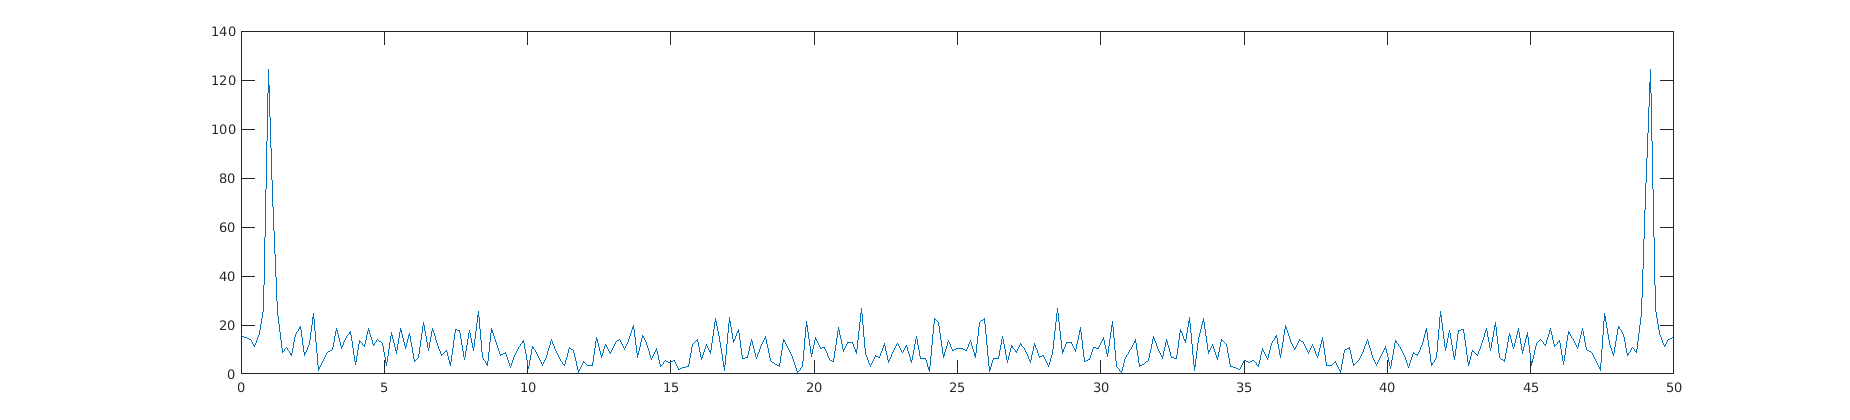
\includegraphics[scale=0.38]{pics/3noise_sin_spec.png}
\caption{Спектр зашумленного сигнала $S$.}
\label{noise_sin_spec}
\end{figure}

\subsection{Фильтрация зашумленного сигнала.}
Для удаления шума из сигнала был синезирован КИХ-фильтр нижних частот 256 порядка. Для этого использован инструмент fdatool, интегрированный в среду MATLAB. Параметры фильтра и его частотная характеристика приведены на Рис. \ref{params}.

\begin{figure}[H]
\centering
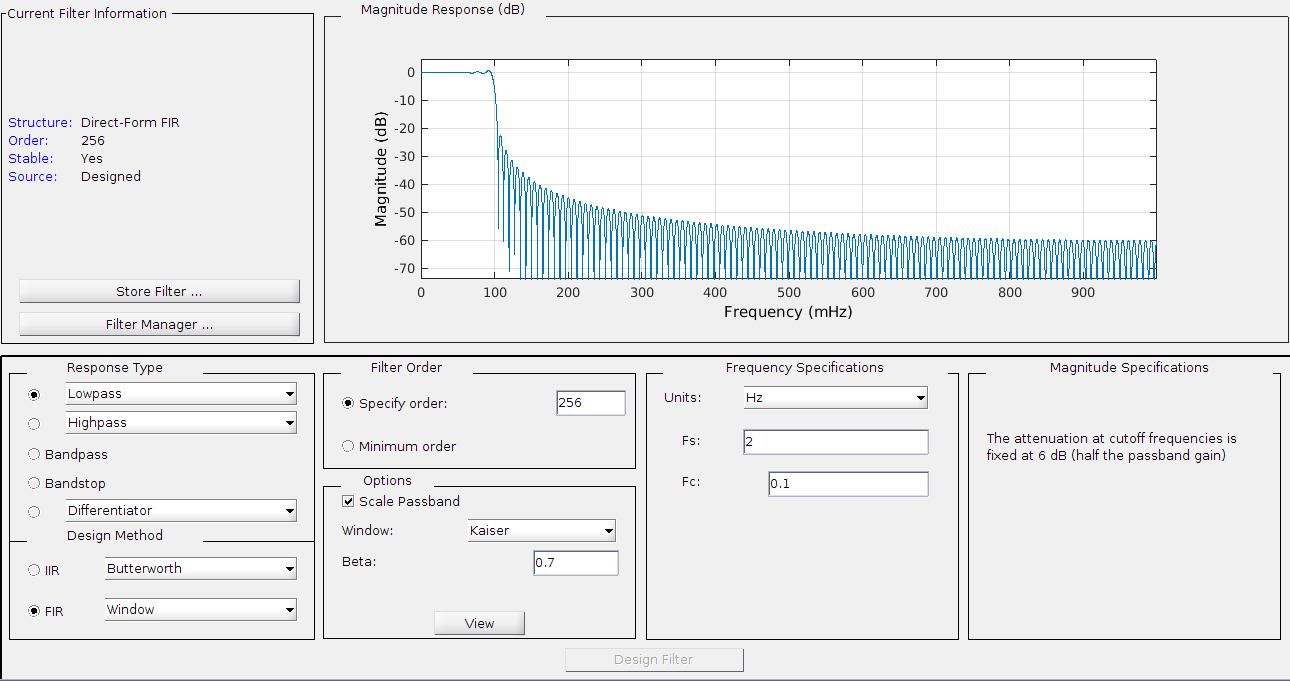
\includegraphics[scale=0.38]{pics/3filter_params.png}
\caption{Параметры синтезированного фильтра.}
\label{params}
\end{figure}

Процесс фильтрации в MATLAB заключается в применении функции filter, которая принимает коэффициенты фильтра и вектор отсчетов входного сигнала, возвращает  отфильтрованный сигнал.

Применим данную функцию к зашумленному сигналу. Результат приведен на Рис. \ref{filtered_1}. На Рис. \ref{filtered_1_spec} -- спектр полученного сигнала.

\begin{figure}[H]
\centering
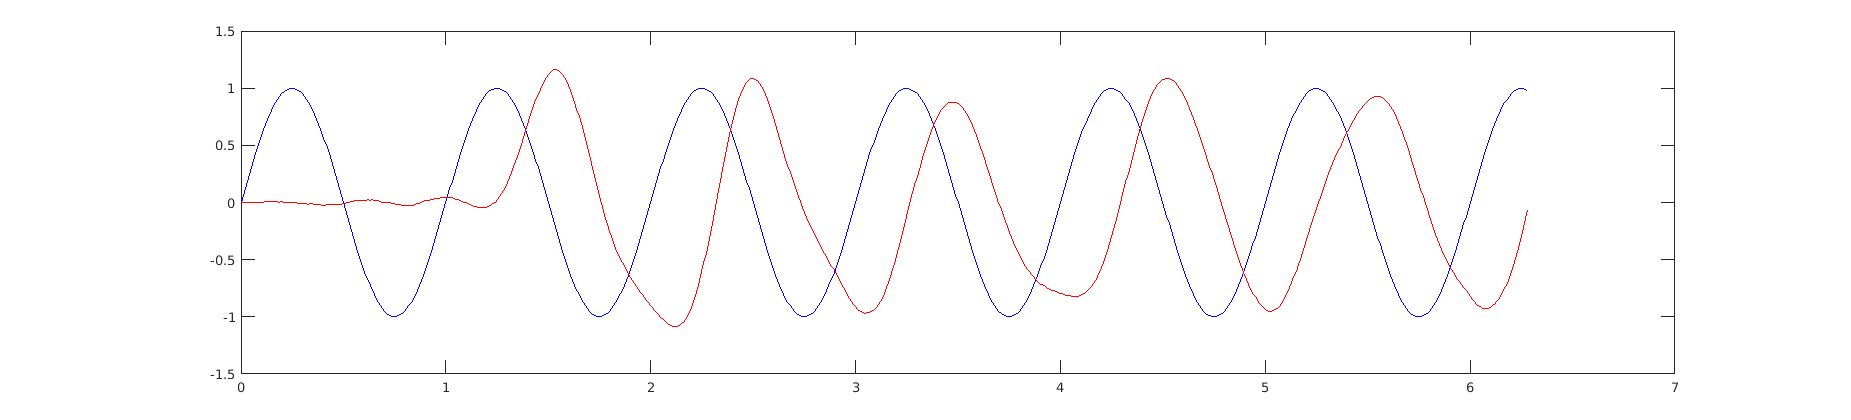
\includegraphics[scale=0.38]{pics/3filtered_3.png}
\caption{Исходный сигнал (синий) и результат работы фильтра (красный).}
\label{filtered_1}
\end{figure}

\begin{figure}[H]
\centering
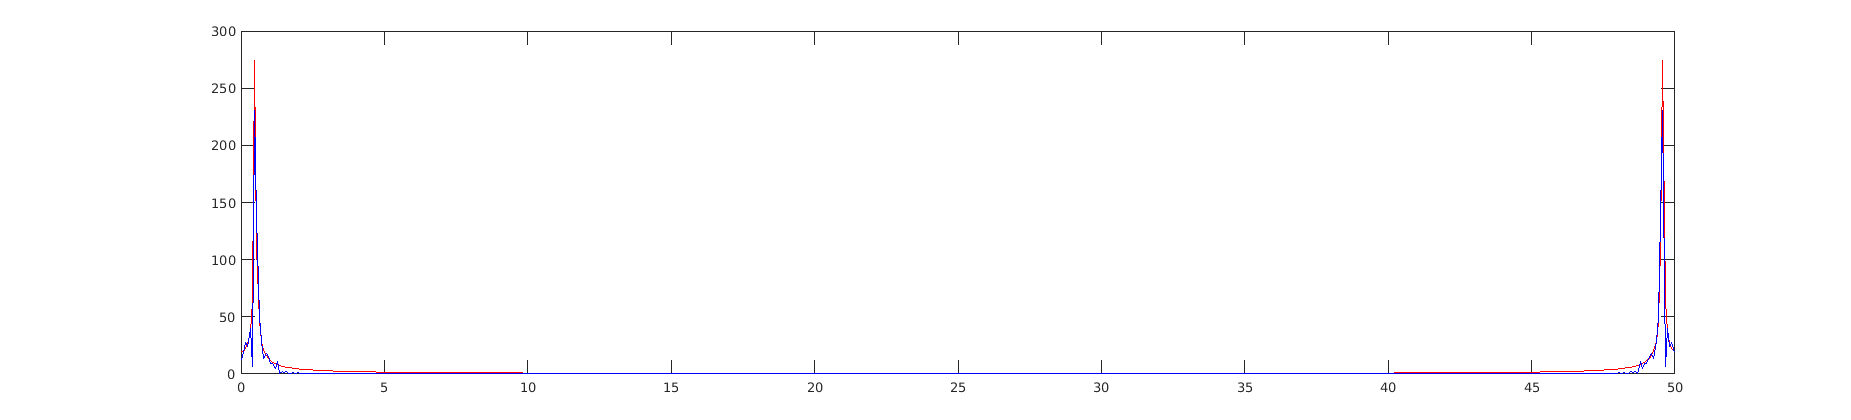
\includegraphics[scale=0.38]{pics/3filtered_3_spec.png} 
\caption{Спектр исходного сигнала (красный) и спектр результата работы фильтра (синий).}
\label{filtered_1_spec}
\end{figure}

Для генерации зашумленного сигнала параметр \textit{snr} был равен 3. Получим еще один зашумленный сигнал с параметром \textit{snr} = -3. Результат фильтрации такого зашуленного сигнала приведен на Рис. \ref{filtered_-3}. Его спектр -- на Рис. \ref{filtered_-3_spec}.

\begin{figure}[H]
\centering
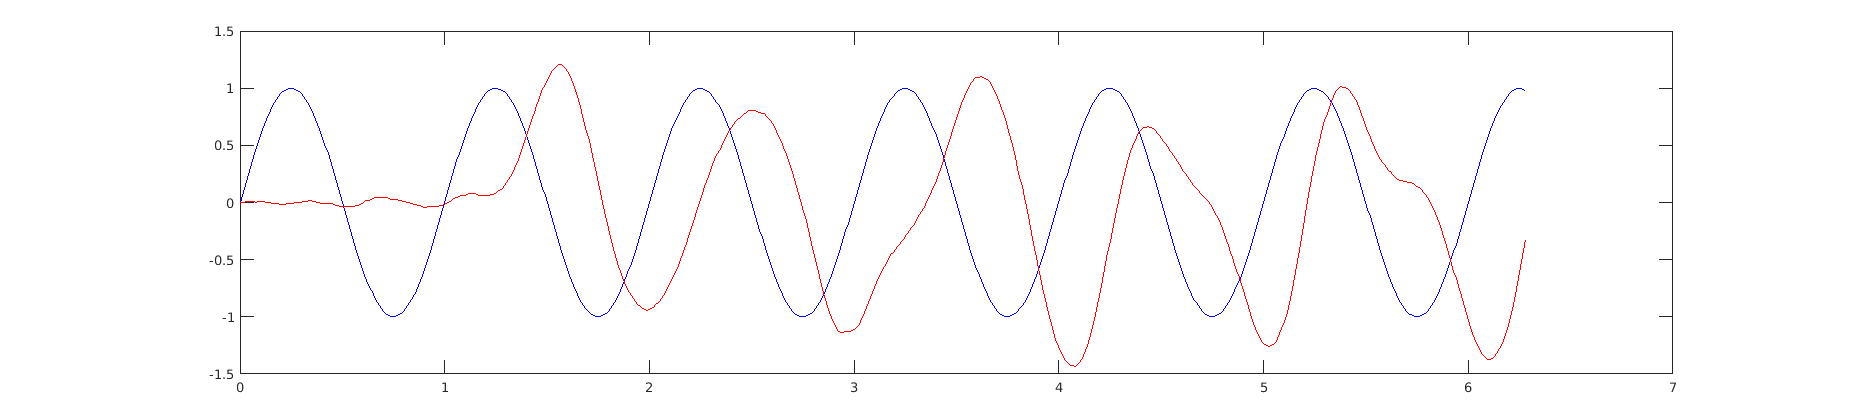
\includegraphics[scale=0.38]{pics/3filtered_-3.png} 
\caption{Исходный сигнал (синий) и результат работы фильтра (красный).}
\label{filtered_-3}
\end{figure}

\begin{figure}[H]
\centering
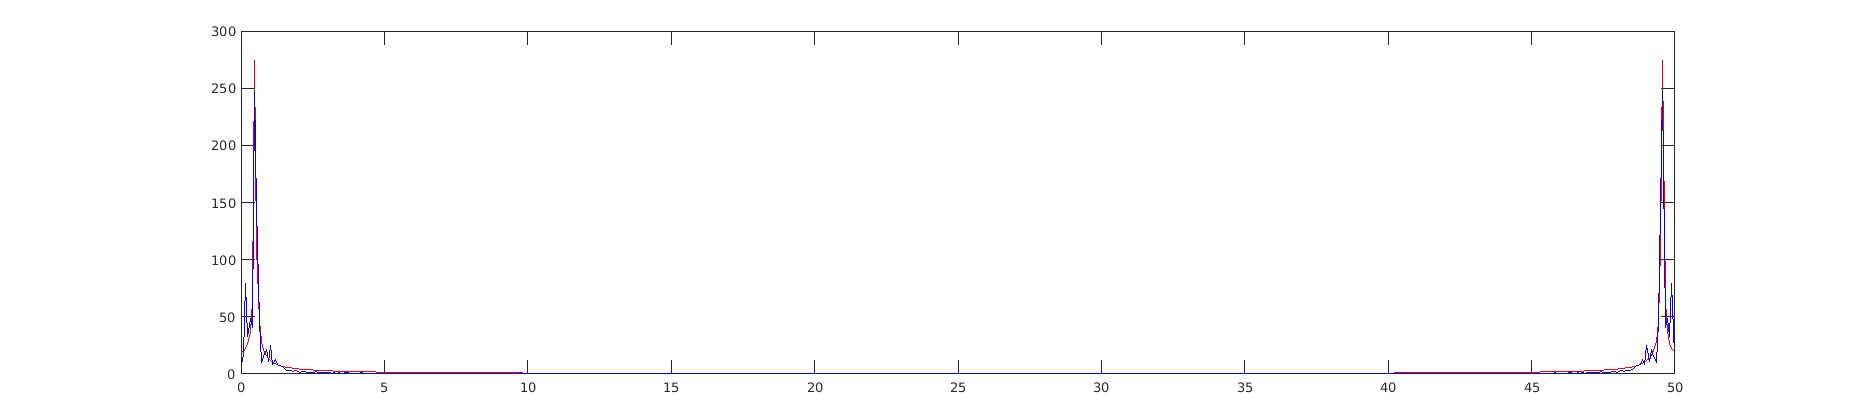
\includegraphics[scale=0.38]{pics/3filtered_-3_spec.png} 
\caption{Спектр исходного сигнала (красный) и спектр результата работы фильтра (синий).}
\label{filtered_-3_spec}
\end{figure}

Полученный отфильтрованный сигнал имеет большие отклонения от исходного.

Изменим параметры фильтра: частоту дискретизации уменьшим с 2 Гц до 1.5 Гц; частоту среза -- с 0.1 Гц до 0.02 Гц:

Результат фильтрации, а также спектр полученного сигнала представлены на Рис. \ref{filtered_-3_changed} и Рис. \ref{filtered_-3_changed_spec}.

\begin{figure}[H]
\centering
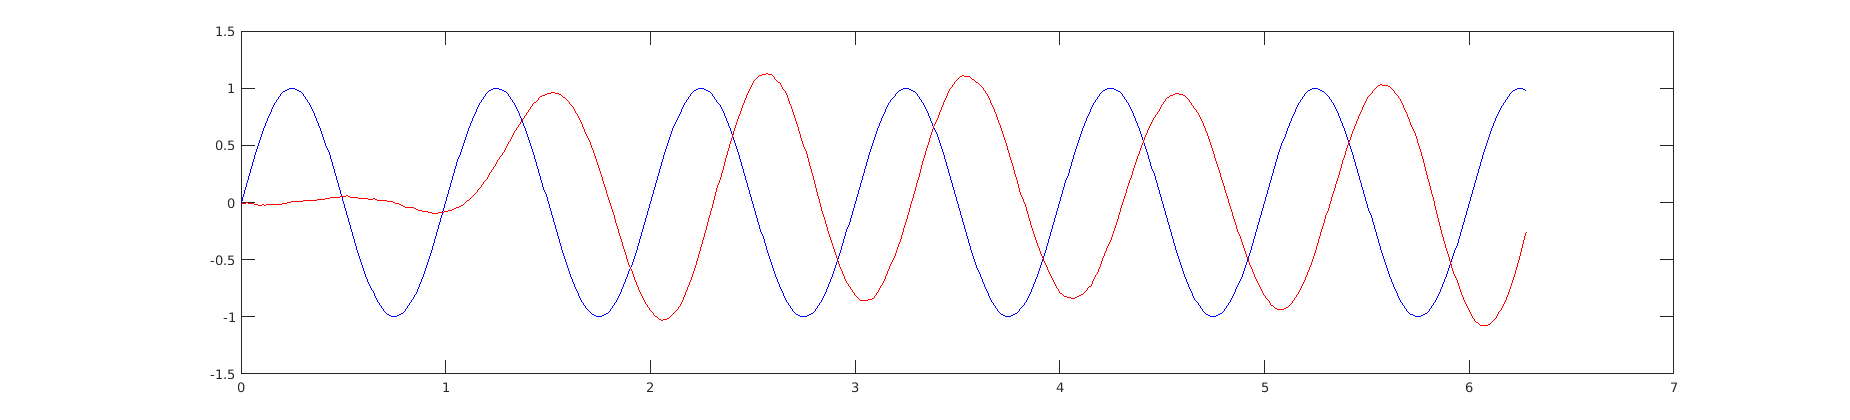
\includegraphics[scale=0.38]{pics/3filtered_-3_changed.png} 
\caption{Исходный сигнал (синий) и результат работы фильтра (красный).}
\label{filtered_-3_changed}
\end{figure}

\begin{figure}[H]
\centering
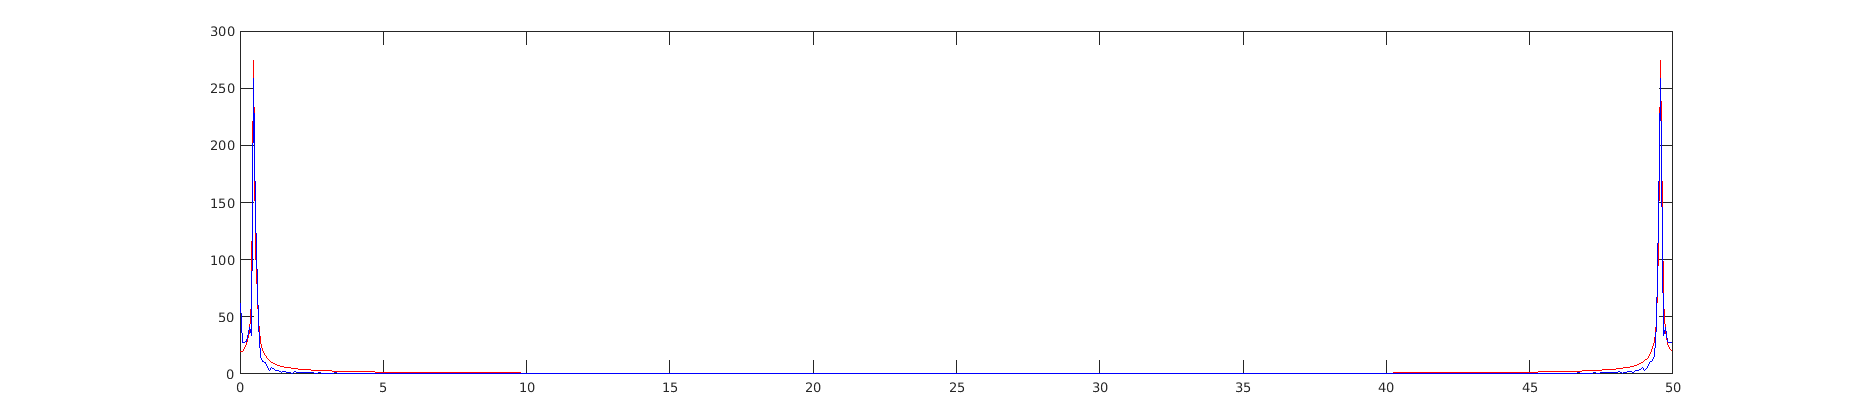
\includegraphics[scale=0.38]{pics/3filtered_-3_changed_spec.png} 
\caption{Спектр исходного сигнала (красный) и спектр результата работы фильтра (синий).}
\label{filtered_-3_changed_spec}
\end{figure}

Видно, что отфильтрованная синусоида стала больше похожа на исходную.

\subsection{Вывод.}
Результат прохождения сигнала через линейную цепь определяется передаточной функцией этой цепи. В случае с линейными фильтрами, спектр сигнала на выходе цепи получается путем умножения спектра входного сигнала на частотную характеристику фильтра. Во временной области этому действию соответствует свертка сигнала с импульсной характеристикой фильтра. 

В данной работе был синтезирован линейный фильтр, рассмотрено прохождение зашумленного гармонического сигнала через него. В результате сигнал был очищен
от высокочастотных шумов. На низких частотах шум удален не был: белый шум имеет сплошной спектр, следовательно, попадает в полосу пропускания фильтра.

\end{document}
